\documentclass[12pt]{article}
        \makeatletter
        \def\input@path{{../../}}
        \makeatother
        \usepackage{sbc-template}
        \makeatletter
        \renewcommand{\inst}[1]{}
        \makeatother
        \usepackage{graphicx,url}
        \usepackage[utf8]{inputenc}
        \usepackage[T1]{fontenc}
        \usepackage[brazil]{babel}
        \usepackage{longtable,booktabs,array}
        \usepackage{amsmath,amssymb}
        \providecommand{\tightlist}{%%
          \setlength{\itemsep}{0pt}\setlength{\parskip}{0pt}}
        \sloppy
        \title{Primeiro pipeline reproduzivel: previsao de demanda no Favorita com baselines e RC}
        \author{}
        \address{}
        \begin{document}

        \maketitle

        \begin{resumo}
        Este artigo transforma a teoria dos dois primeiros capitulos em um pipeline reproduzivel de previsao. O objetivo e ensinar o leitor a executar um baseline forte e um primeiro modelo de Reservoir Computing no mesmo recorte adotado no Favorita, medindo ambos com o mesmo protocolo temporal. Fazemos isso em modo passo-a-passo: carregamos a serie, separamos treino e teste, executamos \texttt{Seasonal\ Naive}, executamos RC, comparamos previsoes, interpretamos metricas e discutimos por que perder para um baseline nao invalida um experimento didatico. O resultado principal e honesto: no recorte inicial, \texttt{Seasonal\ Naive} supera o RC em todas as metricas, mas o RC funciona de ponta a ponta e abre as perguntas certas para os artigos seguintes.
        \end{resumo}

        \subsection{1. O que o leitor vai aprender}\label{1-o-que-o-leitor-vai-aprender}

Ao final deste artigo, voce sera capaz de:

\begin{enumerate}
\def\labelenumi{\arabic{enumi}.}
\tightlist
\item
  executar um pipeline minimo de previsao no Favorita;
\item
  usar \texttt{Seasonal\ Naive} como baseline serio, e nao apenas ilustrativo;
\item
  rodar o RC classico do projeto do inicio ao fim;
\item
  comparar previsoes com as mesmas metricas e o mesmo split temporal;
\item
  interpretar um resultado inicial ruim como parte do processo cientifico.
\end{enumerate}

\subsection{2. O recorte experimental herdado}\label{2-o-recorte-experimental-herdado}

Continuamos usando exatamente o mesmo recorte estabelecido no artigo 1:

\begin{itemize}
\tightlist
\item
  \texttt{store\_nbr\ =\ 1}
\item
  \texttt{family\ =\ BEVERAGES}
\item
  frequencia diaria
\item
  ultimos \texttt{90} dias como teste
\end{itemize}

Isso significa que a comparacao deste artigo e justa por construcao. Ambos os modelos veem os mesmos dados e sao avaliados pelas mesmas metricas.

\subsection{3. Passo 1: carregar a serie e separar treino e teste}\label{3-passo-1-carregar-a-serie-e-separar-treino-e-teste}

O pipeline comeca com as funcoes de \texttt{code/common/favorita.py}.

\begin{verbatim}
config = FavoritaSeriesConfig()
frame = load_store_family_series(store_nbr=config.store_nbr, family=config.family)
train, test = temporal_train_test_split(frame, test_days=config.test_days)
\end{verbatim}

Em notacao temporal, o experimento usa

\[
\mathcal{D}_{train} = \{(x_t, y_t)\}_{t=1}^{T-90},
\qquad
\mathcal{D}_{test} = \{(x_t, y_t)\}_{t=T-89}^T.
\]

Esse split e fundamental. Se ele mudar entre os modelos, a comparacao deixa de ser confiavel.

\subsection{\texorpdfstring{4. Passo 2: executar o baseline \texttt{Seasonal\ Naive}}{4. Passo 2: executar o baseline Seasonal Naive}}\label{4-passo-2-executar-o-baseline-seasonal-naive}

O baseline sazonal do projeto esta em \texttt{code/baselines/seasonal\_naives/model.py} e implementa a regra

\[
\hat{y}_t = y_{t-7},
\]

usando sazonalidade semanal.

A implementacao e curta exatamente porque sua funcao pedagogica e clara:

\begin{verbatim}
pattern = train["y"].to_numpy()[-season_length:]
repeats = int(np.ceil(horizon / season_length))
forecast = np.tile(pattern, repeats)[:horizon]
\end{verbatim}

Para executar:

\begin{verbatim}
python code/baselines/seasonal_naives/run.py
pytest code/baselines/seasonal_naives/test_model.py
\end{verbatim}

Um bom artigo de series temporais nao pula esta etapa. Se um modelo mais sofisticado nao supera esse baseline, isso precisa aparecer no texto.

\subsection{5. Passo 3: executar o primeiro RC}\label{5-passo-3-executar-o-primeiro-rc}

O RC classico do projeto esta em \texttt{code/rc/model.py} e usa a configuracao default:

\begin{itemize}
\tightlist
\item
  \texttt{n\_reservoir\ =\ 80}
\item
  \texttt{spectral\_radius\ =\ 0.6}
\item
  \texttt{leak\_rate\ =\ 0.15}
\item
  \texttt{washout\ =\ 14}
\end{itemize}

A dinamica do reservatorio e

\[
x_t = (1 - \alpha) x_{t-1} + \alpha \tanh(W_{res} x_{t-1} + W_{in} u_t + b),
\]

e o readout resolve uma regressao Ridge sobre

\[
\phi_t = [1; u_t; x_t].
\]

Para executar:

\begin{verbatim}
python code/rc/run.py
pytest code/rc/test_model.py
\end{verbatim}

\subsection{6. Passo 4: medir com o mesmo protocolo}\label{6-passo-4-medir-com-o-mesmo-protocolo}

As quatro metricas usadas na comparacao sao:

\[
\mathrm{MAE},\quad \mathrm{RMSE},\quad \mathrm{WAPE},\quad \mathrm{sMAPE}.
\]

O ponto metodologico aqui e simples, mas decisivo: os modelos precisam ser comparados no mesmo horizonte, com as mesmas observacoes de teste e as mesmas regras de previsao recursiva.

\subsection{7. Resultados iniciais}\label{7-resultados-iniciais}

Os resultados reais obtidos no projeto foram os seguintes.

\begin{longtable}[]{@{}lllll@{}}
\toprule\noalign{}
Modelo & MAE & RMSE & WAPE & sMAPE \\
\midrule\noalign{}
\endhead
\bottomrule\noalign{}
\endlastfoot
Seasonal Naive & 259.067 & 352.280 & 0.1196 & 0.1361 \\
RC & 324.294 & 423.417 & 0.1498 & 0.1653 \\
\end{longtable}

O \texttt{Seasonal\ Naive} supera o RC em todas as metricas. Em particular:

\begin{itemize}
\tightlist
\item
  o \texttt{MAE} do RC ficou 25.2\% acima do baseline sazonal;
\item
  o \texttt{RMSE} do RC ficou 20.2\% acima do baseline sazonal.
\end{itemize}

\pandocbounded{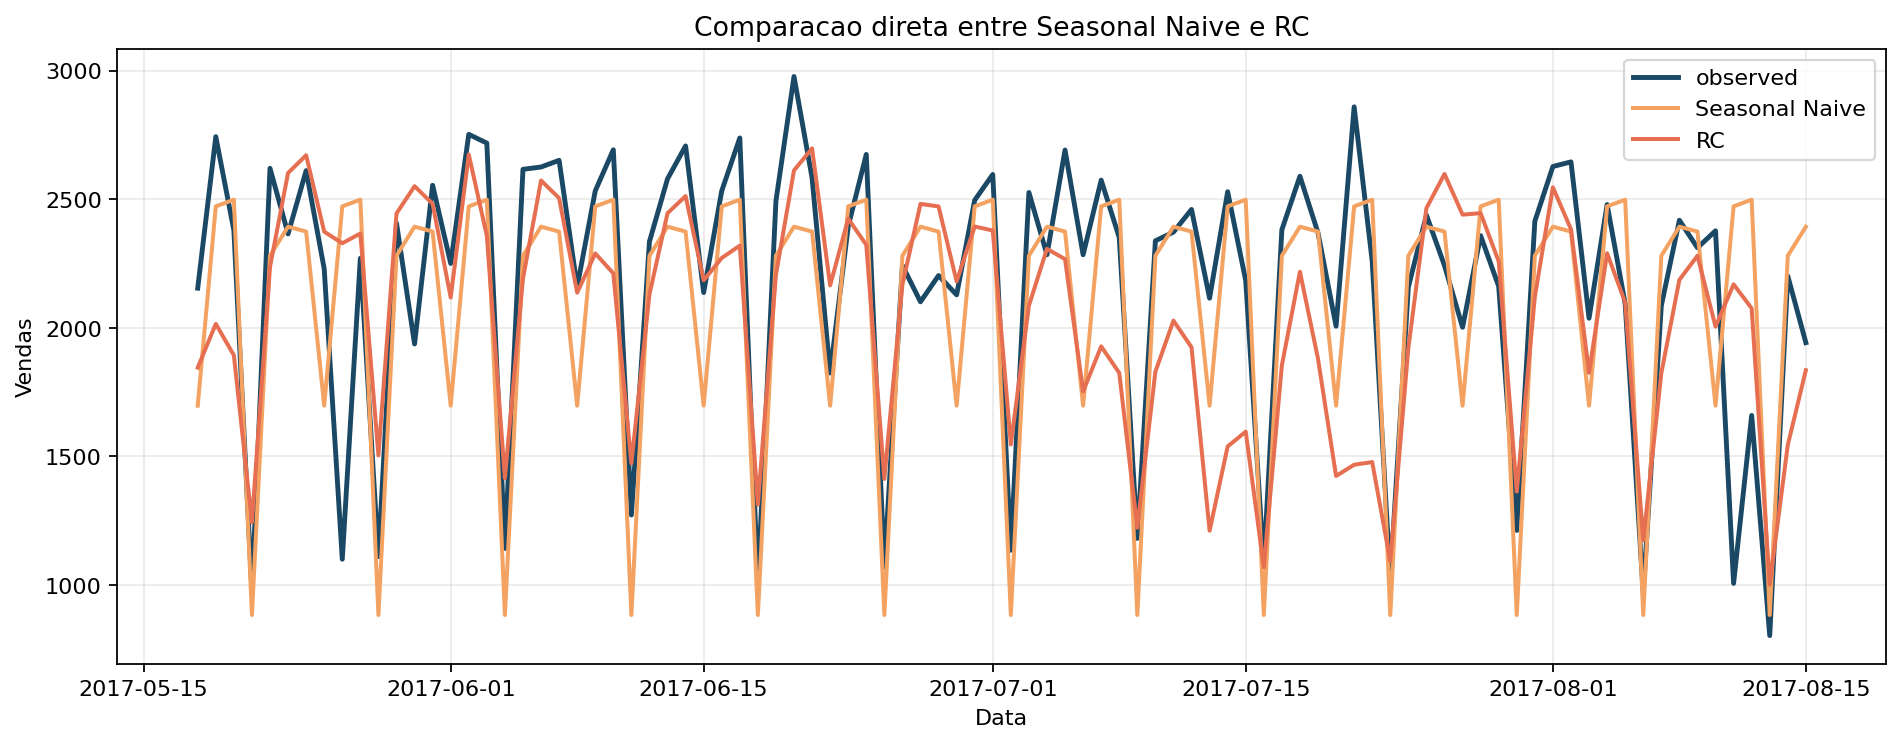
\includegraphics[keepaspectratio,alt={Comparacao direta entre o baseline sazonal e o RC no bloco de teste.}]{computational_results_20260402_222902/baseline_vs_rc_overlay.png}}

A sobreposicao das previsoes ajuda a ler o resultado com mais cuidado do que a tabela numerica isolada:

\begin{itemize}
\tightlist
\item
  o baseline acompanha melhor o padrao semanal;
\item
  o RC funciona, mas ainda oscila mais em torno da serie observada;
\item
  o erro do RC nao vem de um colapso do pipeline, e sim de representacao insuficiente para este primeiro ajuste.
\end{itemize}

\subsection{8. O que este experimento ensina}\label{8-o-que-este-experimento-ensina}

O experimento e didaticamente valioso por quatro motivos.

\subsubsection{8.1 Baseline forte nao e detalhe}\label{81-baseline-forte-nao-e-detalhe}

Em series temporais, um baseline sazonal simples pode ser surpreendentemente competitivo. Isso vale especialmente quando o sinal semanal e forte, como no caso de bebidas no recorte adotado no Favorita.

\subsubsection{8.2 RC nao deve ser tratado como magia}\label{82-rc-nao-deve-ser-tratado-como-magia}

O RC funciona de ponta a ponta: carrega dados, constroi representacao, treina readout e produz previsoes. Mas funcionar nao e o mesmo que vencer. O artigo faz questao de manter essa distincao.

\subsubsection{8.3 Reprodutibilidade e uma conquista em si}\label{83-reprodutibilidade-e-uma-conquista-em-si}

Este pipeline deixa um trilho completo:

\begin{itemize}
\tightlist
\item
  codigo de carregamento;
\item
  execucao do baseline;
\item
  execucao do RC;
\item
  testes;
\item
  metricas salvas;
\item
  imagens comparativas.
\end{itemize}

Essa cadeia e o que permite que os artigos seguintes falem de tuning, avaliacao justa e QRC sem perder a base experimental.

\subsubsection{8.4 Derrota inicial organiza as proximas perguntas}\label{84-derrota-inicial-organiza-as-proximas-perguntas}

Como o RC perdeu para o baseline, os artigos seguintes precisam responder:

\begin{itemize}
\tightlist
\item
  o tamanho do reservatorio esta adequado?
\item
  a memoria do modelo esta curta ou longa demais?
\item
  o raio espectral esta instavel?
\item
  o leak rate esta ajudando ou atrapalhando?
\end{itemize}

Em um bom percurso didatico, resultados fracos produzem perguntas fortes.

\subsection{9. Como este artigo se conecta ao benchmark maior}\label{9-como-este-artigo-se-conecta-ao-benchmark-maior}

O experimento deste artigo nao encerra a comparacao. Ele apenas estabelece o primeiro patamar:

\begin{itemize}
\tightlist
\item
  \texttt{Seasonal\ Naive} sera mantido como referencia;
\item
  RC sera refinado e estudado com mais detalhe;
\item
  novos competidores entrarao depois: \texttt{ETS}, \texttt{Prophet}, \texttt{XGBoost}, \texttt{LSTM} e \texttt{QRC}.
\end{itemize}

Essa progressao e importante porque impede um salto artificial do "primeiro RC" diretamente para o "QRC final".

\subsection{10. Conclusao}\label{10-conclusao}

O primeiro pipeline reproduzivel da serie esta fechado. O baseline sazonal venceu, o RC funcionou sem vencer e o leitor ja tem um experimento concreto para estudar, modificar e rerodar. Isso e exatamente o que um artigo didatico deveria entregar neste ponto: menos promessas vagas e mais reproducao concreta.

O proximo artigo vai usar essa base para explicar por que RC pode melhorar ou piorar tanto quando seus hiperparametros mudam.

\subsection{Entregaveis associados no repositorio}\label{entregaveis-associados-no-repositorio}

\begin{itemize}
\tightlist
\item
  baseline sazonal: \texttt{code/baselines/seasonal\_naives/}
\item
  RC classico: \texttt{code/rc/}
\item
  comparacao numerica e visual deste artigo: \texttt{computational\_results\_20260402\_222902/}
\item
  figuras principais: \texttt{baseline\_vs\_rc\_overlay.png}, \texttt{seasonal\_naive\_forecast\_plot.png}, \texttt{rc\_forecast\_plot.png}
\end{itemize}

\subsection{Referencias}\label{referencias}

\begin{itemize}
\tightlist
\item
  Hyndman, R. J.; Athanasopoulos, G. Forecasting: Principles and Practice.
\item
  Jaeger, H. The "echo state" approach to analysing and training recurrent neural networks.
\item
  Lukosevicius, M. A practical guide to applying echo state networks.
\end{itemize}

        \end{document}
